%!TEX root = ../thesis.tex

\chapter{Evaluation}
\label{cha:evaluation}
In this chapter, I evaluate the web application's fulfillment of the use cases, functional and non-functional requirements specified in Chapter \ref{cha:usecase}. First, I present the different components of the application's graphical user interface. Then, I analyze which parts of the application fulfill which functional requirements. Afterwards, I evaluate the application's user interface according to modern UX design principles. To conclude this chapter, I also provide a short analysis of other non-functional requirements.

\section{Interface Walkthrough}
\label{sec:walkthrough}
\subsection{Start Page}
\begin{figure}
	\centering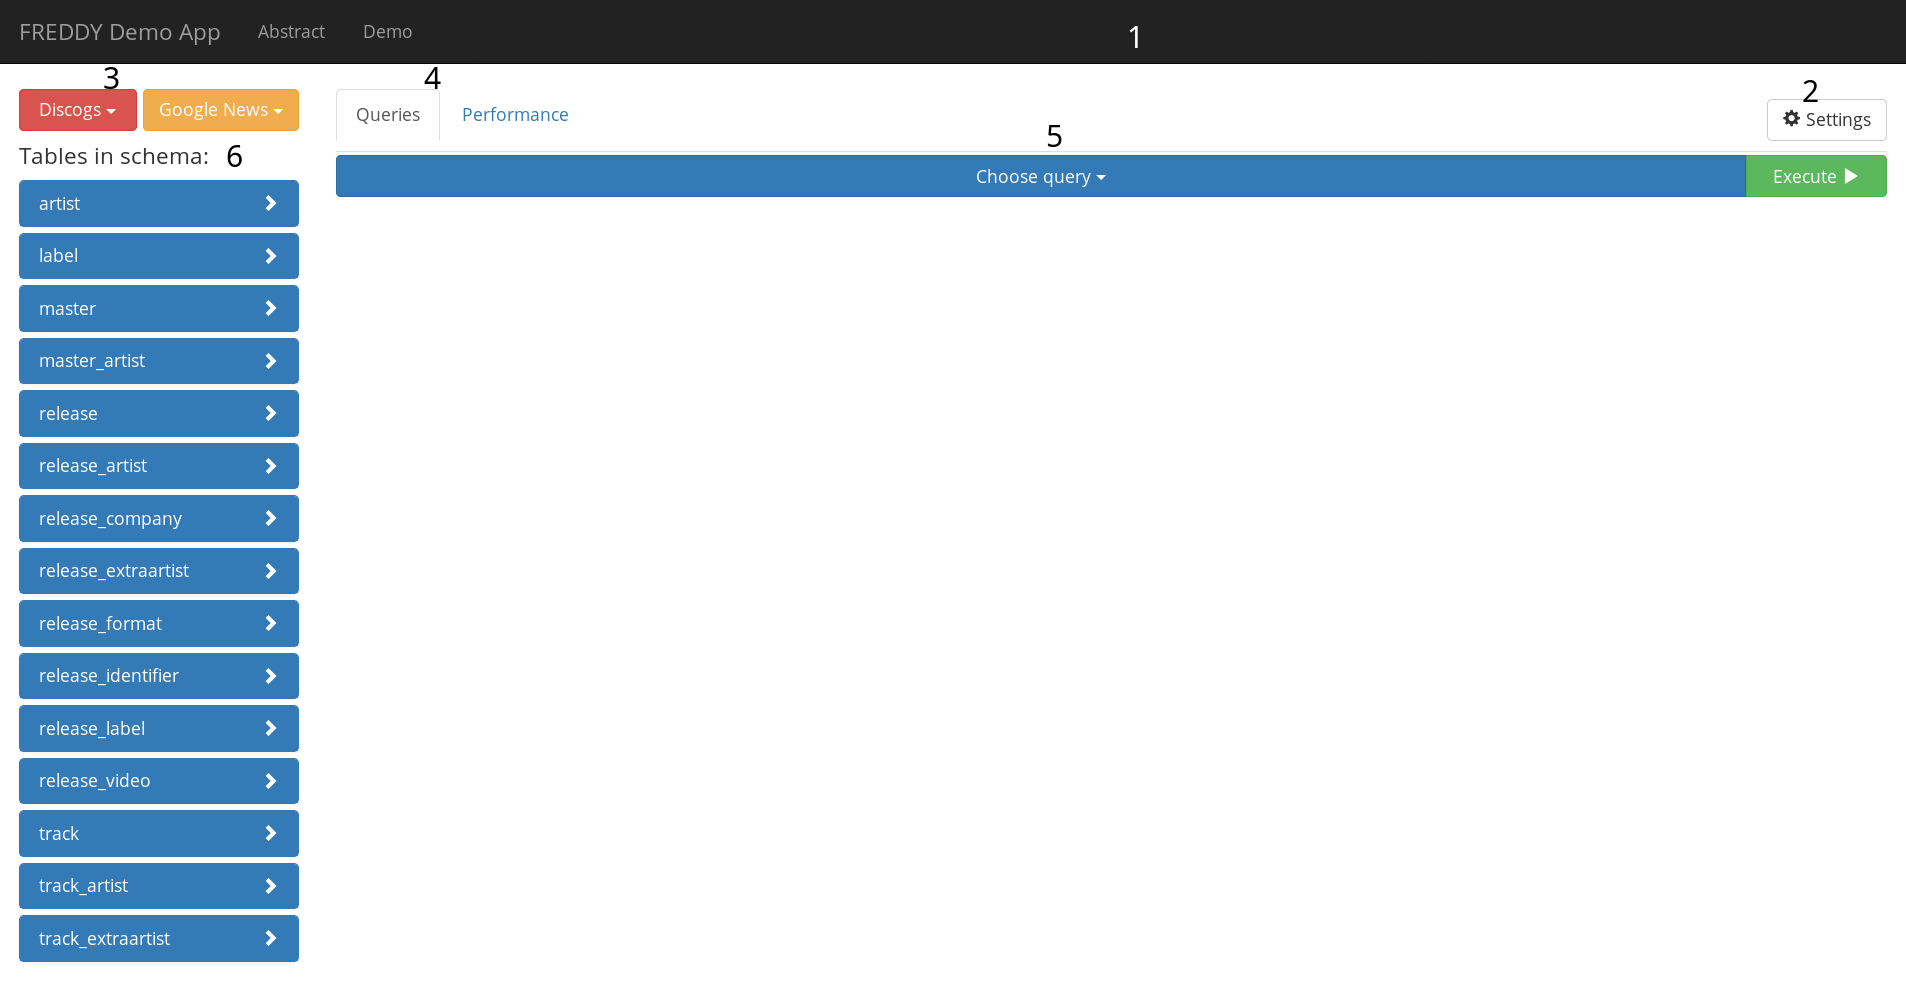
\includegraphics[width=\textwidth,keepaspectratio]{start_page.png}
	\caption{A screenshot of the web application's start page.}
	\label{fig:start_page_screenshot}
\end{figure}
When a user first loads the web application using their web browser, they are greeted by its \textit{start page} (see Figure \ref{fig:start_page_screenshot}). Most of the start page is blank, as results of queries or performance tests are shown in its main part. At the top of it is a navigation bar \textbf{(1)} with the application's name and hyperlinks to the project's abstract and the demo application itself. By default, the demo application is loaded. By clicking on the \textit{Settings} button \textbf{(2)}, the user can show or hide an advanced settings menu. There are two drop-down menus \textbf{(3)} for selecting respectively a database schema to be queried and a word embeddings data set. One can also switch between a database querying view and a word embedding operation performance view by clicking on the respective tab \textbf{(4)}. There is another drop-down menu for selecting a word-embedding-enabled SQL query from a list of predefined queries \textbf{(5)}. On the left of the page, a list of tables in the currently selected schema is displayed \textbf{(6)}. 

\subsection{Settings}
\begin{figure}
	\centering
	\begin{subfigure}[t]{0.6\textwidth}
		\centering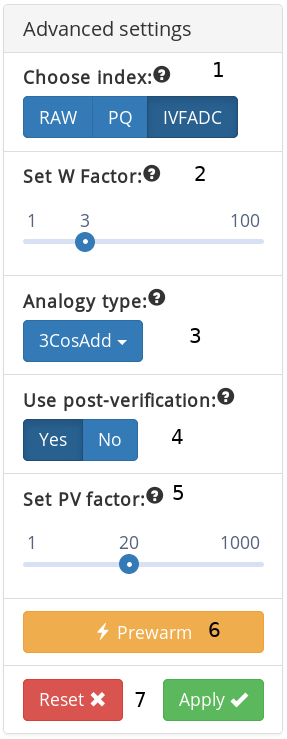
\includegraphics[width=0.55\textwidth,keepaspectratio]{settings.png}
		\caption{A screenshot of the advanced settings menu.}
		\label{fig:settings_menu}
	\end{subfigure}%
	~
	\begin{subfigure}[t]{0.38\textwidth}
		\centering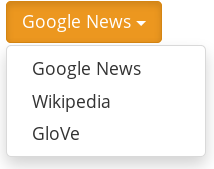
\includegraphics[width=0.6\textwidth,keepaspectratio]{we_picker.png}
		\caption{A screenshot of the word embeddings picker.}
		\label{fig:we_picker}
	\end{subfigure}
	\caption{Screenshots of the front end's settings widgets.}
\end{figure}
\subsubsection{Advanced Settings Menu}
When a user clicks the Settings button, a panel containing widgets for configuring a number of \textit{advanced settings} for FREDDY appears on the right of the page (see Figure \ref{fig:settings_menu}). There is an information tooltip providing the user with a short description of the respective setting for each of the options. The user can choose between raw word embedding operation results or enable the usage of an index \textbf{(1)}. If the user has selected the \textit{IVFADC} index, they can also set the number of nearest coarse quantization clusters considered for a word embedding operation \textbf{(2)}. A drop-down menu \textbf{(3)} allows the selection of one of three analogy function implementations. The user can also enable or disable additional result post-verification \textbf{(4)} and set the number of results to be considered for it by setting the PV factor \textbf{(5)}. The number of results considered for post-verification is equal to the PV factor multiplied by \textit{k} in a k-NN search. By clicking the prewarm button \textbf{(6)}, the user can improve the application's performance immediately after its start by sending a request to FREDDY to load the index tables into the database server's main memory. A pair of buttons \textbf{(7)} allows resetting FREDDY's settings to their defaults and applying the selected settings to the database, respectively. After the settings are applied to the database, they affect all following word embedding operations.

\subsubsection{Word Embeddings Picker}
Using the \textit{word embeddings picker}'s drop-down menu in the top left corner of the page (shown in Figure \ref{fig:we_picker}), the user can select one of three word embeddings data sets to be used in word embedding operations. This affects all following operations, too.

\subsubsection{Schema Picker and Browser}
\begin{figure}
	\centering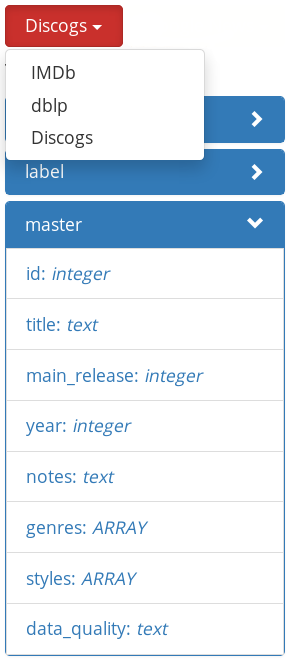
\includegraphics[width=0.3\textwidth,keepaspectratio]{schema_browser.png}
	\caption{A screenshot of the schema picker and browser.}
	\label{fig:schema_picker}
\end{figure}
The leftmost part of the page contains the \textit{schema picker and browser} (shown in Figure \ref{fig:schema_picker}). When a domain-specific data set is selected in the drop-down menu, its schema's tables are displayed as a list below and the list of predefined queries for the specified data set is loaded. Furthermore, when a user clicks on a table's name, a list of columns contained in the table and their datatypes is shown. A user can also conveniently query the data set for the first one thousand values of a specific column by clicking on its name.


\subsection{Query View}
The \textit{query view} is the default view of the web application. It allows the user to send predefined word-embedding-enabled SQL queries to the database, edit them to their preferences and examine their results.

\subsubsection{Query Picker and Editor}
\begin{figure}
	\centering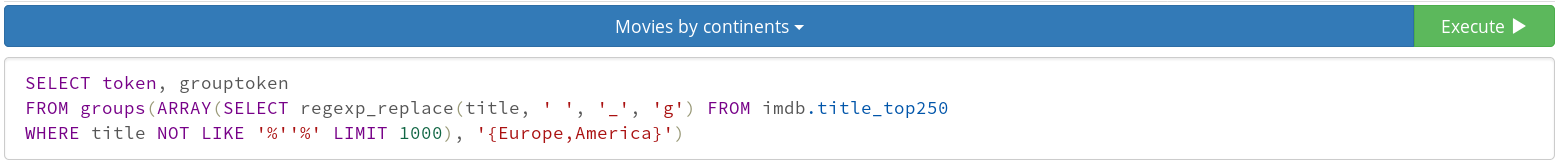
\includegraphics[width=\textwidth,keepaspectratio]{query_editor.png}
	\caption{A screenshot of the query picker and editor.}
	\label{fig:query_picker_editor}
\end{figure}
The query picker and editor are located at the top of the query view (see Figure \ref{fig:query_picker_editor}). The application's user can select a word-embedding-enabled query by its description from a list of predefined queries in the \textit{query picker}'s drop-down menu. After selecting a query, a syntax-highlighted SQL \textit{query editor} appears under the query picker. Here, the user can customize the query to their own liking. After a user is done with editing the query, they can send the query for execution to the database by clicking on the \textit{Execute} button.

\subsubsection{Query Results Table}
\begin{figure}
	\centering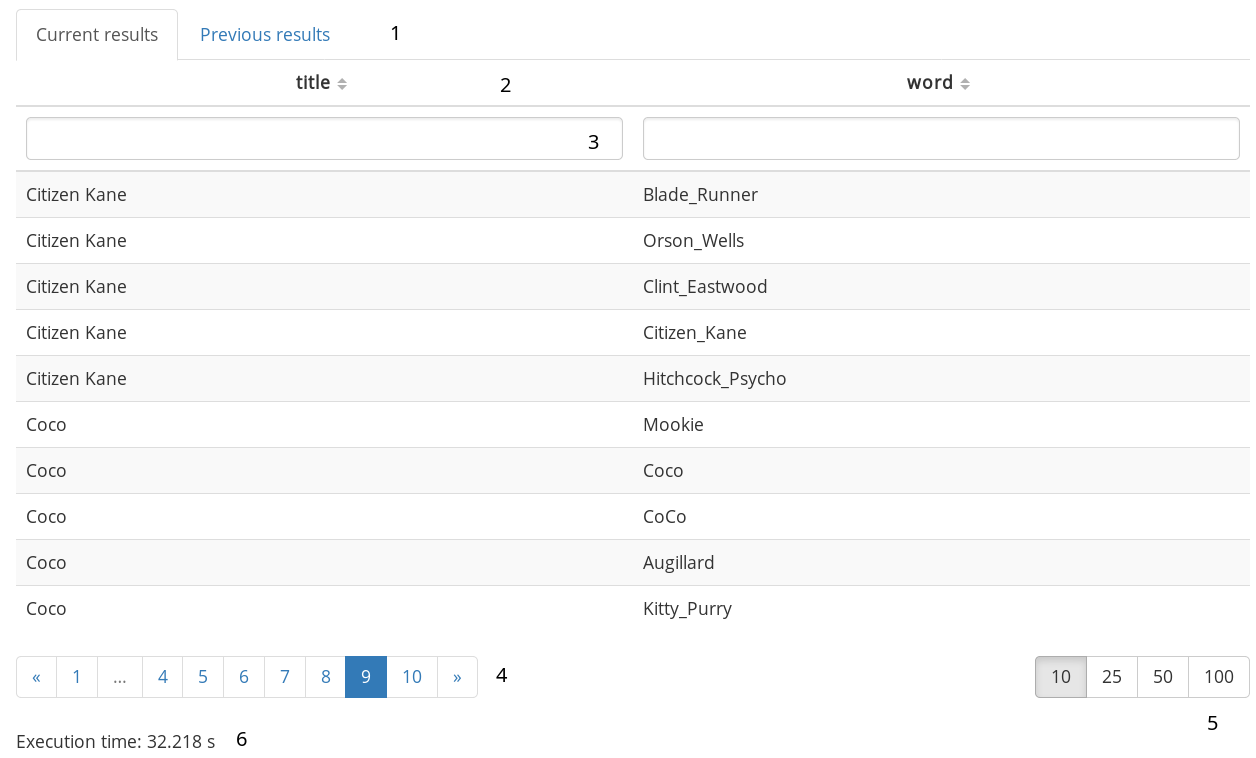
\includegraphics[width=\textwidth,keepaspectratio]{query_results.png}
	\caption{A screenshot of the query results table.}
	\label{fig:query_results}
\end{figure}
The results of a query are displayed in the \textit{query results table} (shown in Figure \ref{fig:query_results}). The user can switch between the results of the previous query and the current one by clicking on the respective tab \textbf{(1)} and sort the result entries in ascending or descending alphanumerical order by clicking on a column's name \textbf{(2)}. Furthermore, options are provided to filter the entries according to a keyword specified by the user \textbf{(3)}. Query results are presented in a number of pages through which the user can browse \textbf{(4)} and they can also adjust the number of entries displayed in a page \textbf{(5)}. Lastly, the query's execution time is shown below the results table \textbf{(6)}. 

\subsection{Performance View}
\begin{figure}
	\centering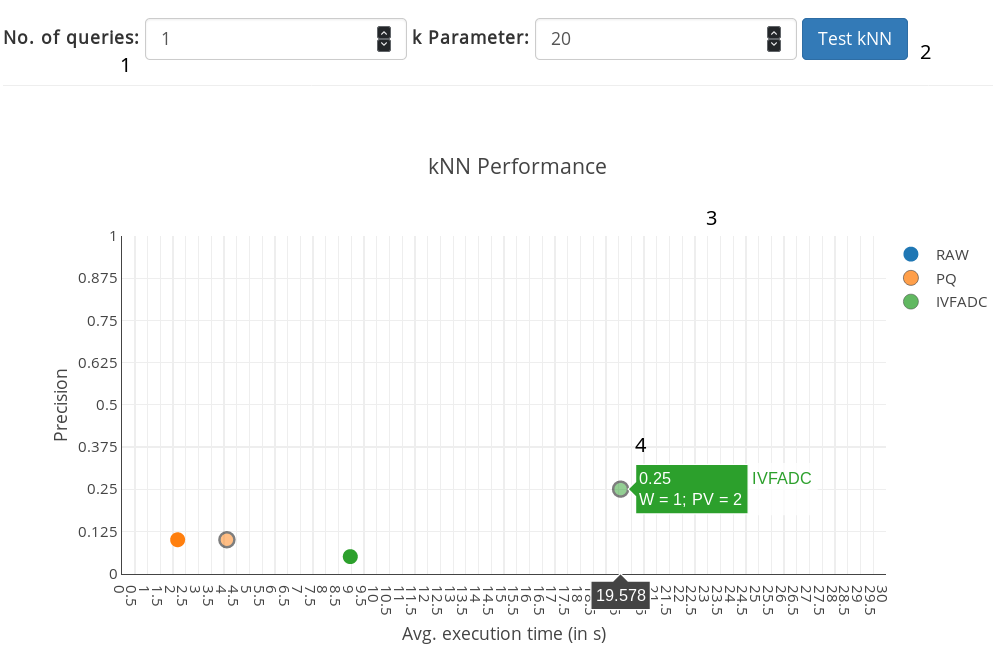
\includegraphics[width=\textwidth,keepaspectratio]{perf_view.png}
	\caption{A screenshot of the performance view.}
	\label{fig:perf_view}
\end{figure}
In the performance view (see Figure \ref{fig:perf_view}), the user can measure the precision and performance of k-NN operations with different parameters. The user can set the parameters for the word embedding operation using the advanced settings menu and can choose the number of operations to be executed and over which the average of the respective metric should be calculated, as well as the parameter \textit{k}, using the provided number boxes \textbf{(1)}. By clicking on the \textit{"Test kNN"} button \textbf{(2)}, the user can initiate the execution of a performance test by the back end. After its completion, a new data point is added to the performance chart \textbf{(3)} which shows the precision (compared to the results of a non-indexed, raw operation) and the average execution time of the operations constituting the performance test. Data points of tests performed using different indexes are shown in a different color and data points of tests using post-verification are displayed semitransparent. Furthermore, when a user place their cursor over a data point, the values of PV and W factors, if they were used in the selected test, are displayed \textbf{(4)}.

\section{Functional Requirements}
\begin{table}
	\centering
	\begin{tabulary}{\textwidth}{|L|L|L|L|}
		\hline
		\textbf{Use Case} & \textbf{Requirement} & \textbf{Involved Components} & \textbf{Interface Part} \\
		\hline
		\textbf{U1} & R1.1 & Front End, Back End, Database & Settings: Schema Picker \\
		\hline
		& R1.2 & Front End, Back End, Queries File & Query View: Query Picker\\
		\hline
		& R1.3 & Front End & Query View: Query Editor \\
		\hline
		& R1.4 & Front End, Back End, Database & Query View \\
		\hline
		& R1.5 & Front End & Query View: Query Results Table \\
		\hhline{|=|=|=|=|}
		\textbf{U2} & R2.1 & Front End, Back End, Database & Schema Browser \\
		\hline
		& R2.2 & Front End, Back End, Database & Schema Browser \\
		\hline
		& R2.3 & Front End & Schema Browser, Query Editor \\
		\hhline{|=|=|=|=|}
		\textbf{U3} & R3.1 & Front End, Back End, Database & Settings: Advanced Settings Menu \\
		\hline
		& R3.2 & ” & ” \\
		\hline
		& R3.3 & ” & ” \\
		\hline
		& R3.4 & ” & ” \\
		\hline
		& R3.5 & ” & Settings: Word Embeddings Picker \\
		\hline
		& R3.6 & Database & n/a \\
		\hhline{|=|=|=|=|}
		\textbf{U4} & R4.1 & Front End, Back End, Database & Performance View \\
		\hline
		& R4.2 & Front End, Back End & n/a \\
		\hline
		& R4.3 & Front End & Performance View \\
		\hline
		& R4.4 & ” & ” \\
		\hline
		& R4.5 & ” & ” \\
		\hline
	\end{tabulary}
	\caption{A table containing an evaluation of the functional requirements for the web application.}
	\label{tab:eval_func_req}
\end{table}
All use cases were tested during the development of the web front end and after its completion. The application fulfills all functional requirements and hence is well-suited for the use cases described in Section \ref{sec:use_case}. Table \ref{tab:eval_func_req} lists which application components and front end interface elements are involved in the fulfillment of a particular functional requirement.

\section{Non-Functional Requirements}
\label{sec:nf_req}
\subsection{User Interface Design [N1]}
In this section, I evaluate the web application's interface according to the \textit{Laws of UX} \cite{laws-of-ux}. Laws of UX is a collection of the maxims and principles that designers can consider when building user interfaces. This list of well-established design laws rooted in psychology was compiled by front-end designer Jon Yablonski in 2018. Currently, seventeen laws are included in the list. I analyze the graphical user interface according to them and comment on the design decisions that were made. Here, I focus only on six of the laws relevant to the web front end's graphical interface. These are the Doherty Threshold \cite{doherty1982economic}, Hick's Law \cite{hick1952rate} \cite{hyman1953stimulus}, Jakob's Law \cite{jakob}, the Laws of Common Region and of Proximity \cite{palmer1992common} and the Zeigarnik Effect \cite{zeigarnik1927behalten}. The short descriptions below quote the Laws of UX website \cite{laws-of-ux}.

\subsubsection{Doherty Threshold}
\begin{quote}
	\textit{"Productivity soars when a computer and its users interact at a pace (<400ms) that ensures that neither has to wait on the other."} 
\end{quote}
The web application's interface by itself is fast and responsive, owing much to the high-performance web frameworks and technologies used. However, its quickness is also heavily dependent on the execution time of the word embedding operations used by it and, consequently, on the performance of the machine on which the database server is deployed. Thus, a user may have to wait up to four minutes for the results of a complex word embedding operation. 

\subsubsection{Hick’s Law}
\begin{quote}
	\textit{"The time it takes to make a decision increases with the number and complexity of choices."} 
\end{quote}
The interface elements' design takes Hick's law into consideration. For instance, only queries and tables of the currently selected schema are shown in the query picker, respectively schema browser. Settings not relevant to the currently selected index and other selected settings are hidden from the user to simplify their choices.

\subsubsection{Jakob’s Law}
\begin{quote}
	\textit{"Users spend most of their time on other sites. This means that users prefer your site to work the same way as all the other sites they already know."}
\end{quote}
For this reason, standard user interface design frameworks and components were used. The Bootstrap framework is used by 17.4 percent of all websites as of June 2018 \cite{bootstrap-stats}, thus its interface components (buttons, radio buttons, text boxes, etc.) should be well-known to most Internet users. Furthermore, other elements of the front end's interface such as sliders for setting a numerical variable's value have been used in graphical user interfaces for decades. I also consulted with several acquaintances who have no prior experience in user interface design to obtain an unbiased opinion about the placement of the \textit{"Apply"} and \textit{"Reset"} buttons in the advanced settings menu in order to determine which option is the most intuitive.

\subsubsection{Law of Common Region and Law of Proximity}
\begin{quote}
	\textit{"Elements tend to be perceived into groups if they are sharing an area with a clearly defined boundary."}
	
	\textit{"Objects that are near, or proximate to each other, tend to be grouped together."} 
\end{quote}
The application of these two laws is evident in the grouping of UI elements according to their common task. For example, the \textit{"Execute"} button is grouped together with the query picker and query editor. The schema picker and schema browser occupy the same area in the interface's left side. The advanced settings menu is clearly defined as a panel, containing all advanced settings in one place. However, it was decided to move the word embeddings data set picker out of the advanced settings menu to the opposite part of the interface in order to expose more of FREDDY's functionality to the user. In this case, functionality was chosen over strict adherence to user interface design principles.

\subsubsection{Zeigarnik Effect}
\begin{quote}
	\textit{"People remember uncompleted or interrupted tasks better than completed tasks."}
\end{quote}
During the application's testing, it became obvious that the lack of visual feedback during a query's execution or after a failed execution leads to the user's confusion about their action's outcome. Therefore, a loading bar showing the progress of the current request was added to the top of the interface. Furthermore, an error message with details about a request's failure appears under the query picker in the event that a query's execution fails. These two additions help the user to track their progress in achieving the respective use case.

\subsection{Separation of Concerns [N2]}
This requirement is fulfilled by the web application's architectural separation in front end, back end and database system, as described in Section \ref{sec:architecture}.

\subsection{Query Execution Performance [N3]}
The performance of the web application's functionalities was measured in two batches of ten consecutive performance tests. In the first one, a standard grouping query was executed using the web application's query view. The query's execution time and the time from the user initiating the query's execution until the loading of the results in the graphical user interface were measured and compared. On average, the web application causes an overhead of 47.9 ms (median 41 ms) over the database-only execution time of a grouping query. \\
The other ten performance tests concern the web application's performance view. Again, the database execution time and the time between the initiation of the k-NN performance test and the update of the performance chart were measured. In each test, ten 5-NN queries were executed at a time. Because of the greater complexity of this scenario, a performance test took 302.4 ms longer on average (median 272 ms) than only the execution of its constituent queries. Both overhead values remain under the Doherty threshold of 400 ms and can be considered negligible for the end user. Furthermore, they do not affect the entire system's performance in a negative way.

\subsection{Web Browser Compatibility [N4]}
The web application's front end was tested using the state-of-the-art (as of June 2018) web browsers Mozilla Firefox (version 60.0.2) and Google Chrome (version 67.0.3396) under the GNU/Linux operating system. No major differences in none of the web application's functionalities, performance or appearance were found.
